    %-------------------------
% Resume in Latex
% Author
% License : MIT
%------------------------

%---- Required Packages and Functions ----

\documentclass[a4paper,11pt]{article}
\usepackage{latexsym}
\usepackage{xcolor}
\usepackage{float}
\usepackage{ragged2e}
\usepackage[empty]{fullpage}
\usepackage{wrapfig}
\usepackage{lipsum}
\usepackage{tabularx}
\usepackage{titlesec}
\usepackage{geometry}
\usepackage{marvosym}
\usepackage{verbatim}
\usepackage{enumitem}
\usepackage[hidelinks]{hyperref}
\usepackage{fancyhdr}
\usepackage{fontawesome5}
\usepackage{multicol}
\usepackage{graphicx}
\usepackage{cfr-lm}
\usepackage[T1]{fontenc}
\setlength{\multicolsep}{0pt} 
\pagestyle{fancy}
\fancyhf{} % clear all header and footer fields
\fancyfoot{}
\renewcommand{\headrulewidth}{0pt}
\renewcommand{\footrulewidth}{0pt}
\geometry{left=1.4cm, top=0.8cm, right=1.2cm, bottom=1cm}
% Adjust margins
%\addtolength{\oddsidemargin}{-0.5in}
%\addtolength{\evensidemargin}{-0.5in}
%\addtolength{\textwidth}{1in}
\usepackage[most]{tcolorbox}
\tcbset{
	frame code={}
	center title,
	left=0pt,
	right=0pt,
	top=0pt,
	bottom=0pt,
	colback=gray!20,
	colframe=white,
	width=\dimexpr\textwidth\relax,
	enlarge left by=-2mm,
	boxsep=4pt,
	arc=0pt,outer arc=0pt,
}

\urlstyle{same}

\raggedright
\setlength{\tabcolsep}{0in}


% Sections formatting
\titleformat{\section}{
  \vspace{-4pt}\scshape\raggedright\large
}{}{0em}{}[\color{black}\titlerule \vspace{-7pt}]

%-------------------------
% Custom commands
\newcommand{\resumeItem}[2]{
  \item{
    \textbf{#1}{\hspace{0.5mm}#2 \vspace{-0.5mm}}
  }
}

\newcommand{\resumePOR}[3]{
\vspace{0.5mm}\item
    \begin{tabular*}{0.97\textwidth}[t]{l@{\extracolsep{\fill}}r}
        \textbf{#1}\hspace{0.3mm}#2 & \textit{\small{#3}} 
    \end{tabular*}
    \vspace{-2mm}
}

\newcommand{\resumeSubheading}[4]{
\vspace{0.5mm}\item
    \begin{tabular*}{0.98\textwidth}[t]{l@{\extracolsep{\fill}}r}
        \textbf{#1} & \textit{\footnotesize{#4}} \\
        \textit{\footnotesize{#3}} &  \footnotesize{#2}\\
    \end{tabular*}
    \vspace{-2.4mm}
}

\newcommand{\resumeProject}[4]{
\vspace{0.5mm}\item
    \begin{tabular*}{0.98\textwidth}[t]{l@{\extracolsep{\fill}}r}
        \textbf{#1} & \textit{\footnotesize{#3}} \\
        \footnotesize{\textit{#2}} & \footnotesize{#4}
    \end{tabular*}
    \vspace{-2.4mm}
}

\newcommand{\resumeSubItem}[2]{\resumeItem{#1}{#2}\vspace{-4pt}}
% \renewcommand{\labelitemii}{$\circ$}
\renewcommand{\labelitemi}{$\vcenter{\hbox{\tiny$\bullet$}}$}
\newcommand{\resumeSubHeadingListStart}{\begin{itemize}[leftmargin=*,labelsep=0mm]}
\newcommand{\resumeHeadingSkillStart}{\begin{itemize}[leftmargin=*,itemsep=1.7mm, rightmargin=2ex]}
\newcommand{\resumeItemListStart}{\begin{justify}\begin{itemize}[leftmargin=3ex, rightmargin=2ex, noitemsep,labelsep=1.2mm,itemsep=0mm]\small}
\newcommand{\resumeSubHeadingListEnd}{\end{itemize}\vspace{2mm}}
\newcommand{\resumeHeadingSkillEnd}{\end{itemize}\vspace{-2mm}}
\newcommand{\resumeItemListEnd}{\end{itemize}\end{justify}\vspace{-2mm}}
\newcommand{\cvsection}[1]{%
\vspace{2mm}
\begin{tcolorbox}
    \textbf{\large #1}
\end{tcolorbox}
    \vspace{-4mm}
}
\newcolumntype{L}{>{\raggedright\arraybackslash}X}%
\newcolumntype{R}{>{\raggedleft\arraybackslash}X}%
\newcolumntype{C}{>{\centering\arraybackslash}X}%
%---- End of Packages and Functions ------

%-------------------------------------------
%%%%%%  CV STARTS HERE  %%%%%%%%%%%
%%%%%% DEFINE ELEMENTS HERE %%%%%%%
\newcommand{\name}{Agus Fuad Mudhofar} % Your Name
\newcommand{\course}{Computer Engineering} % Your Program
% \newcommand{\roll}{xxxxxxx} % Your Roll No.
\newcommand{\phone}{8882111890} % Your Phone Number
\newcommand{\emaila}{agusfuad090@gmail.com} %Email 1

\begin{document}
\fontfamily{cmr}\selectfont
%----------HEADING-----------------
{
  \noindent
\begin{tabularx}{\linewidth}{@{} l L r @{}}
    % Foto
    \raisebox{-0.5\height}{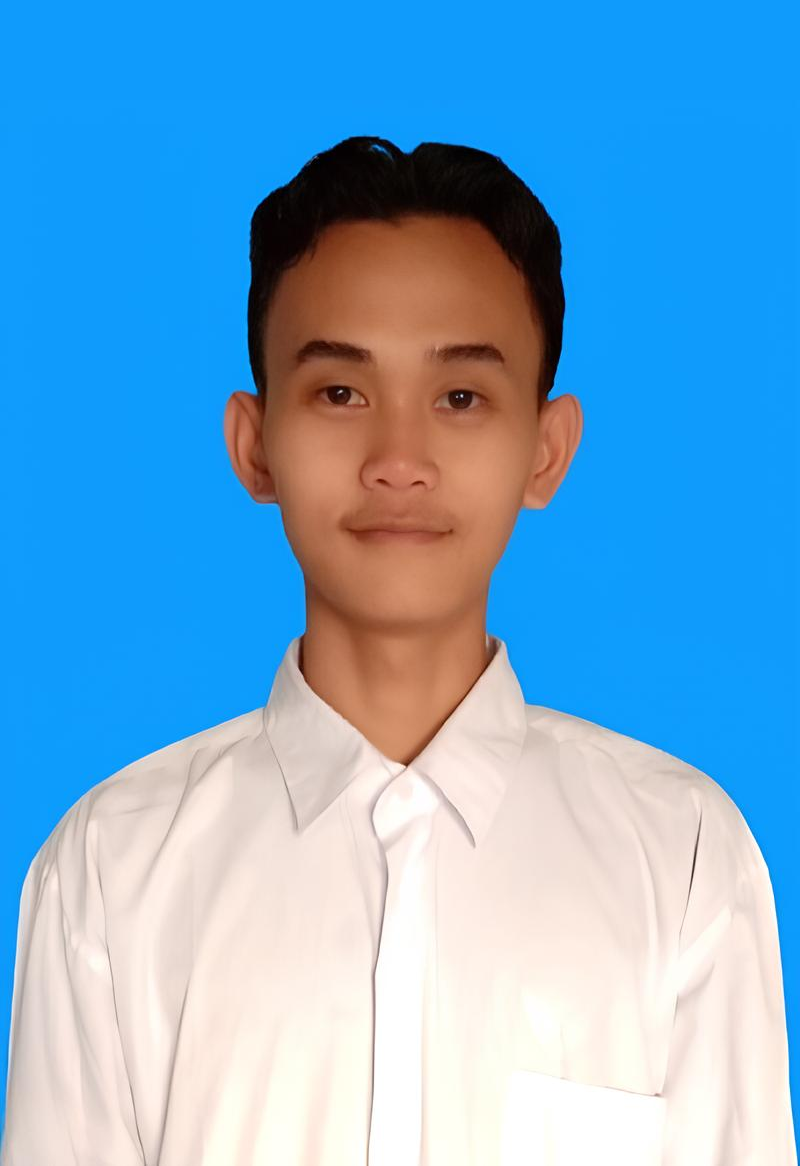
\includegraphics[width=2.5cm]{PAS FOTO Upscale.png}}\hspace{0.5cm} &
    
    % Nama & institusi
    \begin{tabular}[t]{@{}l@{}}
        \textbf{\Large \name} \\
        Institut Teknologi Sepuluh Nopember \\
        Surabaya, Indonesia
    \end{tabular}
    &
    
    % Kontak
    \begin{tabular}[t]{@{}r@{}}
        \raisebox{0.0\height}{\footnotesize \faPhone}\ +62-\phone \\
        \href{mailto:\emaila}{\raisebox{0.0\height}{\footnotesize \faEnvelope}\ \emaila} \\
        \href{https://github.com/MaedaKenji}{\raisebox{0.0\height}{\footnotesize \faGithub}\ GitHub} \\
        \href{https://www.linkedin.com/in/agus4434/}{\raisebox{0.0\height}{\footnotesize \faLinkedin}\ LinkedIn} \\
        NIK: 3207202108040005 \\
        NIM: 5024221021
    \end{tabular}
\end{tabularx}

}

%-----------EDUCATION-----------
\section{\textbf{Pendidikan}}
\resumeSubHeadingListStart
\resumeSubheading
{Teknik Komputer}{IPK: 3.64}
{Institut Teknologi Sepuluh Nopember, Surabaya}{2022-Sekarang}
\resumeSubHeadingListEnd
\vspace{-5.5mm}
%

%-----------PROJECTS-----------------
\section{\textbf{Proyek Pribadi}}
\resumeSubHeadingListStart

\resumeProject
{Smart Wheelchair dengan Kontrol Gerakan Mata} % Project Name
{Sistem kursi roda pintar yang dikendalikan menggunakan mata, mengintegrasikan computer vision dan Embeded System.} % Project Description
{} % Event Dates

\resumeItemListStart
\item {Mengembangkan sistem kursi roda pintar yang memungkinkan pengguna mengontrol pergerakan menggunakan arah pandangan mata, meningkatkan aksesibilitas bagi individu dengan keterbatasan mobilitas.}
\item {Mengintegrasikan pelacakan mata dan pengenalan gestur secara real-time menggunakan Python dan OpenCV, sehingga navigasi dan kontrol menjadi lebih intuitif.}
\item {Mengimplementasikan komponen perangkat keras tertanam (Arduino/ESP32) untuk pengendalian motor dan umpan balik sensor, memastikan operasi yang andal.}
\item {Berkolaborasi dalam tim untuk merancang, membuat prototipe, dan menguji sistem, hingga menghasilkan prototipe fungsional yang dipamerkan pada kompetisi GEMASTIK XVII.}
\item {Teknologi yang Digunakan: Python, OpenCV, Arduino/ESP32, C/C++, algoritma computer vision.}
\resumeItemListEnd
\vspace{-2mm}

\resumeProject
{Sappy: Aplikasi Manajemen Peternakan Multi-Peran (Flutter)} % Project Name
{Aplikasi manajemen peternakan untuk berbagai peran (Peternak, Admin, Dokter) dengan dukungan NFC.}
{} % Event Dates

\resumeItemListStart
\item {Menyediakan akses berbasis peran dan dashboard untuk peternak, administrator, dan dokter dalam satu aplikasi mobile terintegrasi.}
\item {Mendukung bahasa Inggris dan Indonesia menggunakan sistem lokalisasi bawaan.}
\item {Mengimplementasikan manajemen state menggunakan Provider serta fitur NFC untuk identifikasi dan pelacakan yang aman.}
\item {Menyertakan visualisasi data, autentikasi, dan konfigurasi lingkungan menggunakan ekosistem Flutter modern.}
\item {Teknologi yang Digunakan: Flutter, Dart, Provider, NFC, fl\_chart, carousel\_slider, custom fonts/assets.}
\resumeItemListEnd
\vspace{-2mm}

\resumeProject
{Aplikasi Web Pembaca Komik} % Project Name
{Platform web untuk membaca komik yang mendukung manga, manhua, dan manhwa dengan pengalaman membaca yang dioptimalkan.} % Project Description
{} % Event Dates
{}
\resumeItemListStart
\item {Mengembangkan platform pembaca komik yang responsif dengan dukungan manga, manhua, dan manhwa, dilengkapi navigasi halaman yang halus serta optimasi rendering gambar.}
\item {Mengimplementasikan fitur inti seperti manajemen chapter, riwayat baca, autentikasi, dan tata letak adaptif untuk berbagai perangkat.}
\item {Teknologi yang Digunakan: React (frontend), Laravel (backend/API), PostgreSQL (basis data), dengan arsitektur komponen modular dan pengelolaan aset yang dioptimalkan.}
\resumeItemListEnd
\vspace{-2mm}

% ---------------End of Projects
\resumeSubHeadingListEnd
\vspace{-4mm}

% %-----------EXPERIENCE-----------------
\section{\textbf{Pengalaman}}
\resumeSubHeadingListStart
% Start of Experience 1
% \resumeSubheading
% {Web Developer – MIOT Webpage}
% {Laboratorium Multimedia dan IoT (MIOT)}
% {Surabaya}{Ags 2024 - Sekarang}
% \resumeItemListStart
% \item {Merancang dan mengembangkan halaman web resmi Laboratorium MIOT untuk menampilkan riset, publikasi, dan anggota tim.}
% \item {Mengimplementasikan antarmuka pengguna yang responsif dan modern menggunakan React.js dan Tailwind CSS, sehingga dapat diakses dengan baik di berbagai perangkat.}
% \item {Mengintegrasikan manajemen konten dinamis untuk berita, acara, dan profil anggota menggunakan struktur data berbasis JSON.}
% \item {Berkolaborasi dengan anggota laboratorium untuk mengumpulkan kebutuhan, melakukan iterasi desain, serta melakukan deployment situs menggunakan GitHub Pages.}
% \item {Mengoptimalkan performa situs dan SEO, serta menyediakan dokumentasi untuk pemeliharaan dan pengembangan di masa depan.}
% \resumeItemListEnd
% \vspace{-4mm}


% \resumeSubheading
% {Asisten Riset – Laboratorium Multimedia dan IoT (B300)}{Laboratorium Multimedia dan IoT (MIOT)}
% {Surabaya}{April - Juni 2025}
% \resumeItemListStart
% \item {Melakukan riset terkait penerapan model deep learning pada perangkat edge menggunakan NVIDIA Jetson Nano dengan fokus pada tugas computer vision.}
% \item {Mengembangkan dan mengoptimalkan pipeline deteksi objek menggunakan Python dan C++ dengan arsitektur MobileNet-SSD, YOLOv5n, dan YOLOv11s.}
% \item {Mengeksplorasi teknik konversi dan akselerasi model menggunakan ONNX dan NVIDIA TensorRT untuk inferensi real-time.}
% \item {Mengintegrasikan dan mengevaluasi model dalam NVIDIA DeepStream SDK untuk analisis video yang efisien dan siap di-deploy.}
% \item {Melakukan benchmarking performa dan penggunaan sumber daya untuk mengoptimalkan kecepatan inferensi dan akurasi pada lingkungan dengan keterbatasan sumber daya.}
% \resumeItemListEnd
% \vspace{-2mm}


\resumeSubheading
{Asisten Praktikum – Pemrograman Dasar}{Laboratorium Multimedia dan IoT (MIOT)}
{Surabaya}{Ags 2025 - Nov 2025}
\resumeItemListStart
\item {Mengembangkan dan memelihara modul praktikum, termasuk latihan pemrograman dan panduan troubleshooting, serta bertanggung jawab dalam deployment dan pemeliharaan website \textit{online judge} DMOJ yang digunakan dalam perkuliahan.}
\item {Membimbing mahasiswa dalam pengerjaan tugas praktikum bahasa C/C++, memberikan dukungan teknis dan penjelasan secara langsung.}
\item {Mengevaluasi hasil tugas mahasiswa, memberikan umpan balik konstruktif, serta berkontribusi dalam penyusunan rubrik penilaian untuk memastikan evaluasi yang adil dan konsisten.}
\item {Menyelenggarakan dan memimpin sesi review sebelum ujian, membahas miskonsepsi umum dan memperkuat konsep pemrograman inti.}
\resumeItemListEnd
\vspace{-2mm}

% \resumeSubheading
% {Asisten Praktikum – Sistem Digital}{Laboratorium Robotika dan Sistem Digital (B401)}
% {Surabaya}{Mar 2025 - Mei 2025}
% \resumeItemListStart
% \item {Melaksanakan sesi praktikum mata kuliah \textit{Rangkaian Digital}, mendukung lebih dari 100 mahasiswa sarjana setiap semester.}
% \item {Mengembangkan dan memelihara materi praktikum, termasuk skema perangkat keras dan panduan troubleshooting untuk eksperimen logika digital.}
% \item {Membimbing mahasiswa dalam tugas desain rangkaian digital, memberikan dukungan teknis dan penjelasan secara real-time.}
% \item {Berkolaborasi dengan dosen untuk meningkatkan alur kerja praktikum, mengimplementasikan alat bantu pembelajaran baru, serta meningkatkan pengalaman belajar secara keseluruhan.}
% \item {Menyelenggarakan dan memimpin sesi review sebelum ujian, membahas miskonsepsi umum dan memperkuat konsep utama sistem digital.}
% \resumeItemListEnd
% \vspace{-2mm}

% \resumeSubheading
% {Asisten Praktikum – Workshop Telematika}{Laboratorium Robotika dan Sistem Digital (B401)}
% {Surabaya}{Mar 2025 - Mei 2025}
% \resumeItemListStart
% \item {Menyiapkan dan mengembangkan modul praktikum serta materi instruksional untuk \textit{Workshop Telematika}, memastikan pembelajaran berbasis praktik yang terstruktur bagi mahasiswa.}
% \item {Mengawasi dan membimbing mahasiswa selama sesi laboratorium, khususnya pada aktivitas berbasis perangkat keras seperti penyolderan manual, desain 3D untuk prototipe, penyolderan hot air (blower), reflow soldering, dan pencetakan 3D.}
% \item {Memberikan bantuan teknis secara real-time dalam pemrograman C/C++ dan eksperimen berbasis mikrokontroler, membantu mahasiswa dalam menyelesaikan permasalahan perangkat lunak maupun perangkat keras.}
% \item {Menilai hasil praktikum mahasiswa, memberikan umpan balik konstruktif, serta berkontribusi dalam penyusunan kriteria penilaian untuk memastikan evaluasi yang adil dan konsisten.}
% \item {Menyelenggarakan dan memimpin sesi review sebelum penilaian, memperkuat pemahaman konsep utama dan keterampilan praktis.}
% \resumeItemListEnd

% \resumeSubheading
% {Asisten Workshop – International Workshop on Deep Learning}
% {Institut Teknologi Sepuluh Nopember}{Surabaya}
% {24 - 29 Nov 2025}

% \resumeItemListStart
% \item {Membantu pelaksanaan workshop internasional selama 5 hari yang berfokus pada aplikasi machine learning dan deep learning untuk teknologi asistif.}
% \item {Memberikan dukungan langsung kepada peserta dengan membantu menyelesaikan kendala teknis dan kesulitan pembelajaran selama sesi workshop.}
% \item {Mendukung dosen dan pembicara dalam pelaksanaan acara, termasuk koordinasi administratif dan tugas logistik di lokasi.}
% \item {Berkontribusi dalam menciptakan lingkungan belajar yang inklusif dan suportif bagi mahasiswa dari Malaysia, Vietnam, Filipina, Ethiopia, Pakistan, dan Indonesia.}
% \resumeItemListEnd

\resumeSubHeadingListEnd
\vspace{-5.5mm}


% -----------POSITIONS OF RESPONSIBILITY-----------
\section{\textbf{Leadership Experience}}
\resumeSubHeadingListStart
\resumeSubheading
{Ketua Tim – GEMASTIK XVII (Divisi IoT)}
{Universitas Negeri Semarang (UNNES)}{Semarang}
{Jan - Nov 2024}

\resumeItemListStart
\item {Memimpin tim yang mewakili Institut Teknologi Sepuluh Nopember pada Divisi Piranti Cerdas, Sistem Benam, dan IoT di ajang GEMASTIK XVII.}
\item {Mengoordinasikan pekerjaan tim pada komponen perangkat lunak dan perangkat keras, mengelola timeline, serta membagi tanggung jawab secara efektif.}
\item {Mengembangkan sistem kursi roda pintar yang dapat dikendalikan melalui pergerakan mata dengan mengintegrasikan computer vision dan perangkat keras tertanam.}
\item {Meraih penghargaan Finalis Nasional (Juara Harapan) melalui perencanaan, perumusan ide, dan eksekusi inovasi berbasis IoT secara efisien.}
\resumeItemListEnd
\vspace{-4mm}

\resumeSubheading
{Kepala Departemen Logistik – Multimedia and Game Event (MAGE X)}
{Multimedia and Game Event (MAGE X)}
{Surabaya}{Jan - Nov 2024}
\resumeItemListStart
\item {Memimpin tim logistik untuk MAGE X, sebuah ajang kompetisi multimedia dan game tingkat universitas.}
\item {Mengoordinasikan pengadaan, manajemen inventaris, serta distribusi perlengkapan dan peralatan acara.}
\item {Menyusun dan mengeksekusi perencanaan logistik untuk memastikan persiapan tepat waktu dan kelancaran operasional di berbagai lokasi acara.}
\item {Berkolaborasi dengan departemen lain untuk menangani kebutuhan mendadak dan menyelesaikan tantangan logistik selama acara berlangsung.}
\item {Mengelola hubungan dengan vendor, pencatatan anggaran, serta rekonsiliasi inventaris pasca-acara.}
\resumeItemListEnd
\vspace{-4mm}
\resumeSubHeadingListEnd


% -----------ORGANIZATIONAL EXPERIENCE-----------
\section{\textbf{Pengalaman Organisasi}}
\resumeSubHeadingListStart
\resumeSubheading
{Ketua Divisi Web – Laboratorium Multimedia dan IoT (MIOT)}
{Institut Teknologi Sepuluh Nopember}{Surabaya}{2025 - Sekarang}
\resumeItemListStart
\item {Mengelola dan memimpin divisi web dalam laboratorium multimedia dan IoT, bertanggung jawab atas pengembangan situs web dan aplikasi berbasis web.}
\item {Mengkoordinasikan proyek-proyek pengembangan web dengan tim teknis lainnya.}
\item {Menyusun dokumentasi teknis dan memberikan pelatihan kepada anggota tim baru.}
\resumeItemListEnd

% \resumeSubheading
% {Anggota – UKM Rebana ITS}
% {Institut Teknologi Sepuluh Nopember}{Surabaya}{2022 - 2023}
% \resumeItemListStart
% \item {Menjadi anggota aktif dalam unit kegiatan mahasiswa musik tradisional universitas dengan fokus pada pertunjukan Rebana.}
% \item {Berpartisipasi dalam berbagai acara budaya untuk menampilkan musik tradisional serta mempromosikan warisan budaya.}
% \item {Berkolaborasi dengan sesama anggota dalam menyelenggarakan latihan, pertunjukan, dan kegiatan pengabdian kepada masyarakat.}
% \item {Menjadi Ketua Proyek Welcome Party 2022; mengorganisasi kegiatan untuk menyambut dan mengintegrasikan mahasiswa baru ke dalam UKM Rebana ITS.}
% \resumeItemListEnd

\resumeSubheading
{Staf Ahli – UKM Rebana ITS}
{Institut Teknologi Sepuluh Nopember}{Surabaya}{2023 - 2024}
\resumeItemListStart
\item {Menjabat sebagai staf ahli dalam unit kegiatan mahasiswa musik tradisional universitas, memberikan arahan dan kepemimpinan dalam pertunjukan Rebana.}
\item {Memimpin latihan serta berkontribusi dalam penyelenggaraan acara budaya dan kompetisi, guna mempromosikan musik tradisional dan warisan budaya.}
\item {Membimbing anggota junior dan membantu menjaga keberlanjutan tradisi budaya di UKM Rebana ITS.}
\resumeItemListEnd
\resumeSubHeadingListEnd

% -----------SKILLS-----------------
\section{\textbf{Soft Skill}}
\begin{itemize}[leftmargin=0.05in, label={}]
  \small{\item{
        \textbf{Kepemimpinan}{: Kemampuan kepemimpinan yang kuat, dikembangkan melalui pengalaman memimpin tim dalam kegiatan akademik maupun non-akademik.} \\
        \textbf{Komunikasi}{: Kemampuan komunikasi dan presentasi yang efektif, diperoleh melalui workshop, kegiatan, dan kolaborasi tim.} \\
        \textbf{Pemecahan Masalah}{: Kemampuan berpikir analitis dan pemecahan masalah yang terasah melalui proyek teknis dan kegiatan riset.} \\
        }}
\end{itemize}
\vspace{-16pt}

\section{\textbf{Hard Skill}}
\begin{itemize}[leftmargin=0.05in, label={}]
  \small{\item{
        \textbf{Bahasa Pemrograman}{: C/C++, Python, JavaScript, HTML+CSS, Go } \\
        \textbf{Library}{: C++ STL, Python Libraries, ReactJS }\\
        \textbf{Alat Pengembangan Web}{: Node.js, VS Code, Git, GitHub } \\
        \textbf{Framework}{: ReactJS, Laravel} \\
        \textbf{Cloud/Basis Data}{: MongoDB, Firebase, Basis Data Relasional (MySQL) } \\

        \textbf{Mata Kuliah Relevan}{: Struktur Data \& Algoritma, Sistem Operasi, Pemrograman Berorientasi Objek, Sistem Manajemen Basis Data, Pemrograman Mobile } \\
        \textbf{Bidang Minat}{: Pengembangan Perangkat Lunak} \\
        }}
\end{itemize}
\vspace{-16pt}

\end{document}
